%% IPM --- Elsevier elsarticle (authors in frontmatter under the title; titlepage mirrors the same block)
\documentclass[preprint,12pt,authoryear]{elsarticle}

\usepackage{amssymb,amsmath}
\usepackage{graphicx}
\usepackage{booktabs}
\usepackage{multirow}
\usepackage{array}
\usepackage{xurl}
\usepackage{microtype}
\usepackage{placeins}
\usepackage{float}
\usepackage{lineno}
\usepackage{algorithm}
\usepackage{algpseudocode}
\usepackage{amsthm}
\usepackage[hidelinks]{hyperref}
\newtheorem{definition}{Definition}
\newtheorem{proposition}{Proposition}
\newtheorem{remark}{Remark}
\graphicspath{{figures/}}
\DeclareUrlCommand\codeid{\urlstyle{tt}}
\newcommand{\tbd}{---}
% Compact tables: never stretch with \resizebox (avoids oversized, eye-catching grids).
\newcommand{\compacttab}{\setlength{\tabcolsep}{4.5pt}\renewcommand{\arraystretch}{1.05}}

\journal{Information Processing \& Management}

\begin{document}

\begin{frontmatter}

\title{BIMS-LEGAL: Dual-Store Soft Binding for Recovering Prior Legal Advice under Same-Domain Interference}

%% Author names and affiliations appear under the title (IPM/Elsevier frontmatter),
%% not at the end of the article. End-matter CRediT is a contribution statement only.
\author[uw]{Linrui Xu}
\ead{xu-l81@webmail.uwinnipeg.ca}
\author[lab,idl]{Linrui Han\corref{cor1}}
\ead{linrui_han@163.com}
\cortext[cor1]{Corresponding author. Postal address: No.~25 Xitucheng Road, Haidian District, Beijing 100088, China.}
\affiliation[uw]{organization={University of Winnipeg},
            addressline={515 Portage Avenue},
            city={Winnipeg},
            postcode={R3B 2E9},
            state={Manitoba},
            country={Canada}}
\affiliation[lab]{organization={Ministry of Education Laboratory of Philosophy and Social Sciences -- The CUPL Data Law Lab, China University of Political Science and Law},
            addressline={No.~25 Xitucheng Road, Haidian District},
            city={Beijing},
            postcode={100088},
            country={China}}
\affiliation[idl]{organization={The Institute for Data Law, China University of Political Science and Law},
            addressline={No.~25 Xitucheng Road, Haidian District},
            city={Beijing},
            postcode={100088},
            country={China}}

\begin{abstract}
\sloppy
In same-domain legal consultation archives, dense retrieval often surfaces a relevant client question while failing to return the lawyer's advice turn---an \emph{episode incompleteness} failure that leaves prior recommendations hard to recover under lexical interference from neighbouring matters.
BIMS-LEGAL indexes Chinese consultation logs in a dual store: a fast episodic turn index with session identifiers and a slower BIRCH semantic store.
Soft~O2 binds session siblings by attenuated score inheritance ($\beta s$) rather than hard score copy.
Exact replay is reported only as a surface-form reference; the main channels are paraphrase, follow-up, and advice-recall.
On a shared turn-level index Soft~O2 improves over dense FlatIP, with hard hydration and shuffled-$sid$ controls separating binding from score copying and membership noise.
Gains are largest where a partial episode hit can pull in its answer sibling.
Soft~O2-C and gated Hybrid extend binding to BIRCH clusters under a Mix protocol with off-session gold; when query and gold already share a session, Soft~O2 is preferred.
We report Answer Hit, Episode Completeness, graded nDCG with fixed gold-session IDCG, a complete/incomplete/miss failure taxonomy, and paired significance tests.
\end{abstract}

\begin{keyword}
legal information retrieval \sep consultation memory \sep soft episode binding \sep dual-store memory \sep cluster binding \sep Chinese legal corpora
\end{keyword}

\end{frontmatter}

\linenumbers

\section{Introduction}\label{sec:intro}

A junior associate may ask a firm assistant: ``Last month you advised this client on terminating a fixed-term contract---what remedy did we recommend?'' The system returns several near-identical ``contract termination'' questions, ranks the stored user utterance highly, and never surfaces the partner's written advice. The subsequent reply may sound fluent yet be grounded in the wrong episode---or in none. In consultation archives, questions and answers share specialized terminology; neighbouring matters are topically adjacent yet legally distinct; and the professionally useful evidence unit is the full consultation \emph{episode}.

Legal informatics has long studied statutory interpretation, case retrieval, and advisory systems \cite{martinezgil2023survey, ashley2017artificial}.
Recent legal large language models (LLMs) improve statutory and fact-pattern answering \cite{yue2023disclawllm, huang2023lawyer, yue2024lawllm}.
Classical legal information retrieval (IR) mainly targets \emph{external} authority---statutes, cases, or community answers---as documents \cite{askari2024legalqa, louis2024lleqa, liu2022query, zhang2024event}.
Memory-augmented dialogue systems recover evidence from evolving conversation logs \cite{wu2025longmemeval, maharana2024evaluating, packer2023memgpt}.
The gap addressed here is \emph{internal consultation memory}: retrieving prior client-specific advice from a growing same-domain archive under lexical interference.

BIMS-LEGAL (Brain-Inspired Memory System for legal consultation archives) separates a fast episodic pathway---timestamped turn embeddings with speaker role and session identifier $sid$---from a slow semantic pathway based on Balanced Iterative Reducing and Clustering using Hierarchies (BIRCH) with deferred consolidation \cite{zhang1996birch}.
Complementary Learning Systems (CLS) theory \cite{mcclelland1995complementary, kumaran2016} is used only as an architectural analogy for that dual-pathway split.
Under same-domain interference, dense turn retrieval in a vector database often returns a question turn while its answer sibling remains outside top-$k$---a system-level episodic memory failure we term \emph{episode incompleteness}, distinct from a full session miss and exacerbated by IVFPQ score collapse and context fragmentation at moderate archive sizes.

The \emph{algorithmic contributions} are soft binding operators that complete episodes without hard score copy:
\begin{itemize}
    \item \textbf{Soft~O2 (session soft binding).} When a turn is retrieved with score $s$, siblings sharing $sid$ inherit $\max(s_{t'},\,\beta\cdot s)$, surfacing answer turns under question-hit~/~answer-miss while preserving rank competition among candidates.
    \item \textbf{Soft~O2-C and gated Hybrid (cluster soft binding).} The same soft-inheritance rule applies within BIRCH clusters when gold evidence is not co-session with the query; Hybrid triggers cluster binding only on direct dense hits to avoid displacing same-session siblings.
\end{itemize}
Two \textbf{implementation operators} support large shared-store experiments but are not standalone algorithmic contributions:
\begin{itemize}
    \item \textbf{O1 (exact FlatIP indexing).} At hundreds-to-thousands of turns, IVFPQ product quantization is under-trained and collapses Answer Hit; FlatIP restores faithful turn scores so Soft~O2 inherits uncorrupted sibling signals.
    \item \textbf{O3 (bulk-load consolidation).} Deferred BIRCH and disk writes make archive construction tractable without changing retrieval semantics.
\end{itemize}

We ask four research questions:

\begin{itemize}
    \item \textbf{RQ1.} Under same-domain interference, how prevalent is episode incompleteness (question hit~/~answer miss) relative to full session miss?
    \item \textbf{RQ2.} Do Soft~O2 and Soft~O2-C address episode incompleteness under measured index distortion, and what incremental gains does Soft~O2 provide over FlatIP and hard parent hydration?
    \item \textbf{RQ3.} On the \emph{same} LegalEp~/LegalMem stores, when is the slow (BIRCH) pathway effective? Does Soft~O2-C help under standard same-session gold, and under a fair Mix of same-/cross-session gold?
    \item \textbf{RQ4.} Across CAIL multi-turn and LegalEp paraphrase~/advice-recall channels, how large and session-tied are Soft~O2 gains, and when do Soft~O2-C~/Hybrid help beyond Soft~O2?
\end{itemize}

\paragraph{Contributions.}
\begin{enumerate}
    \item A dual-store memory architecture for Chinese legal consultation archives, separating fast episodic turn recovery from slower BIRCH semantic integration under same-domain interference.
    \item Soft~O2, a turn-level session soft-binding operator that recovers missing answer siblings without hard parent hydration or session-max score copy.
    \item A three-candidate score-competition account of Soft~O2 using the gap ratio $\rho=s_d/s_h$, with default $\beta{=}0.98$ chosen by validation sweep.
    \item Turn-level lexical and fusion controls (BM25-turn, dense+BM25 RRF, cross-encoder) under the same evidence unit as Soft~O2, with joint episode indexing treated as a coarser alternative design rather than a turn-binding baseline.
    \item Soft~O2-C and gated Hybrid on Mix cross-session reconstructions, graded nDCG with fixed gold-session IDCG, a failure taxonomy, and paired significance tests.
    \item O1 exact FlatIP and O3 bulk-load consolidation as implementation operators for the shared-store ablations.
\end{enumerate}

Section~\ref{sec:related} reviews related work.
Section~\ref{sec:method} presents BIMS-LEGAL operators and the Soft~O2 attenuation analysis.
Section~\ref{sec:protocol} details corpora, metrics, and protocols.
Section~\ref{sec:experiments} reports results.
Section~\ref{sec:discussion} discusses implications and limitations.
Section~\ref{sec:conclusion} concludes.

\section{Related Work}\label{sec:related}

\subsection{Legal IR and long-horizon dialogue memory}
Legal QA and retrieval systems typically ground generation in statutes, cases, or published advice \cite{louis2024lleqa, askari2024legalqa, martinezgil2023survey, ashley2017artificial}.
Conversational legal case retrieval and event-aware similar-case ranking further show how interaction context and structured legal knowledge shape IR effectiveness \cite{liu2022query, zhang2024event}.
Those pipelines optimize access to external authority.
Consultation memory retrieval targets a different evidence source: \emph{prior consultation episodes} inside an agent's own archive.
Confusing two clients' histories can produce fluent yet professionally inappropriate responses even when statute retrieval is correct.
Domain LLMs such as DISC-LawLLM, Lawyer~LLaMA, and LawLLM improve statutory and advisory generation \cite{yue2023disclawllm, huang2023lawyer, yue2024lawllm}, but they still need a reliable memory index when prior advice must be recovered from a growing same-domain log.

Legal consultation archives add a further difficulty: high lexical overlap among topically adjacent matters, with the professionally useful evidence unit being the full question--answer episode.
This setting motivates \emph{dual-store} memory architectures that keep fast episodic turn retrieval separate from slower semantic clustering, and session-aware soft binding operators that recover answer turns under same-domain interference without collapsing rank competition among unrelated candidates.

\subsection{Dual-store memory and episodic retrieval}
Dual-store designs distinguish fast episodic encoding from slower semantic integration \cite{mcclelland1995complementary, kumaran2016, tulving1972episodic, atkinson1971control}.
Memory architectures for dialogue agents extend context via hierarchical paging, summary banks, graphs, and neuro-symbolic retrieval \cite{packer2023memgpt, zhong2024memorybank, rasmussen2025zep, gutierrez2024hipporag, modarressi2023ret, wang2024memoryllm, lewis2020rag, wu2025memory}, but most treat retrieved units as flat passages rather than \emph{multi-turn consultation episodes} whose answer turn may rank below an unrelated question turn sharing legal vocabulary.
LongMemEval and LoCoMo evaluate long-horizon recall and QA over personal conversation logs \cite{wu2025longmemeval, maharana2024evaluating}, while broader memory-agent surveys emphasize persistence beyond the context window \cite{wu2025memory, Tan2025}.
Recent conversational RAG work stresses reuse of historical search evidence across turns \cite{mo2026historical}.
BIMS-LEGAL positions its dual-store contribution at this intersection: episodic turn embeddings with $sid$ for same-session recovery (Soft~O2), and BIRCH centroids with Soft~O2-C for cross-session recovery when query and gold evidence occupy different sessions but share thematic structure \cite{zhang1996birch}.
Under dense same-domain interference, a question turn can occupy top-$k$ while its answer sibling is absent.
Parent-document hydration and session-max aggregation recover that sibling by hard score copy; Soft~O2 instead injects attenuated inherited scores so episode completion does not erase rank competition among unrelated candidates.

\subsection{Session-aware retrieval}
Parent-document hydration, session aggregation, and joint session indexing are standard session-aware mechanisms for attaching sibling context to a dense hit.
Soft episode binding (Soft~O2) inherits $\beta\cdot s$ for siblings and keeps ranking competition among candidates. Parent-document and hierarchical retrieval similarly attach child evidence to a parent unit \cite{callan1994passage,dai2019context,zaheer2017deep,karpukhin2020dpr}; Soft~O2 differs by using attenuated turn-level score propagation rather than hard hydration or atomic session documents.
Lexical BM25 \cite{robertson2009bm25}, dense passage retrieval \cite{karpukhin2020dpr}, dense--sparse Reciprocal Rank Fusion \cite{cormack2009rrf}, and cross-encoder reranking \cite{nogueira2019multistage, chen2024bge} provide complementary controls outside session membership.
Exact flat indexes and product-quantized ANN backends \cite{johnson2019billion} further affect whether sibling binding is applied over faithful turn scores.

\paragraph{Contrast with joint-episode indexing.}
An alternative way to keep episode context is to concatenate full question--answer pairs into monolithic episode documents (joint indexing).
Joint indexing can prevent episode incompleteness by construction, but it changes the evidence unit from individual turns to merged documents.
That coarser unit weakens fine-grained turn matching---for example, isolating a specific advice sentence---and raises index memory and update cost when new turns arrive in an online consultation log.
Soft~O2 instead keeps turn-level representations and candidate competition, recovering missing siblings on demand via attenuated score inheritance ($\beta s$) without replacing the underlying turn index.
Table~\ref{tab:rw_compare} summarizes the session-structure contrasts used in the main grids.

\begin{table}[htbp]
\centering
\caption{Session-aware mechanisms compared in this work.}
\label{tab:rw_compare}
\compacttab\footnotesize
\begin{tabular}{@{}llp{2.2cm}cc@{}}
\toprule
\textbf{Mechanism} & \textbf{Unit} & \textbf{Expansion} & \textbf{Type} & \textbf{Rank} \\
\midrule
Parent hydration & Session & Insert siblings & Hard & No \\
Session-max & Session & Session $\max$ & Hard & Same$^*$ \\
Joint episode index & Session doc & Atomic & N/A & N/A \\
Soft O2 & Turn+$sid$ & Soft $\beta s$ & Soft & Yes \\
Soft O2-C & Turn+cluster & Soft $\beta_c s$ & Soft & Yes \\
\bottomrule
\end{tabular}
\end{table}
{\footnotesize $^*$On the reported corpora, session-max rankings coincide with hard parent hydration under full-sibling expansion; main tables report a single hard-expansion baseline. Soft~O2 denotes session soft binding; Soft~O2-C denotes cluster soft binding on the BIRCH pathway.}

In short, the dual-store split is the system design, and Soft~O2~/Soft~O2-C are the operators evaluated on Chinese legal consultation archives.

\section{Method: BIMS-LEGAL}\label{sec:method}

\subsection{Architecture overview}
Figure~\ref{fig:bims_architecture} summarizes the pipeline.
BIMS-LEGAL maintains complementary episodic and semantic stores over the same consultation archive.

\begin{definition}[Episodic and semantic elements]\label{def:elements}
An \emph{episodic turn} (episodic element) is $e_i=(\mathbf{v}_i,t_i,c_i,\phi_i,sid_i)$, where $\mathbf{v}_i\in\mathbb{R}^d$ is an embedding, $t_i$ a timestamp, $c_i$ conversational context (including speaker role), $\phi_i$ surface features, and $sid_i$ the consultation session identifier.
We reserve \emph{session turns} for the weaker notion of turns that share only $sid$ under a grouping key, without requiring role, timestamp, or other episodic metadata to participate in scoring.
Soft~O2 binds over session siblings $\mathrm{Sib}(t)=\{t':sid_{t'}=sid_t\}\setminus\{t\}$, but the indexed objects themselves remain episodic turns.
A semantic element is $s_j=(\mathbf{c}_j,C_j,\kappa_j,\tau_j)$ with centroid $\mathbf{c}_j$, member set $C_j$, label $\kappa_j$, and formation statistics $\tau_j$.
Write $\mathrm{Clus}(t)=\{t':cid_{t'}=cid_t\}\setminus\{t\}$ for BIRCH-cluster siblings.
\end{definition}

\begin{definition}[Dual-store retrieval map]\label{def:retrieval}
Given query $q$ with embedding $\mathbf{v}_q$, base episodic retrieval returns a scored candidate set $\mathcal{R}_0(q)=\{(t,s_t)\}$ under Eq.~\eqref{eq:base-score}.
Soft~O2 produces $\mathcal{R}_{\mathrm{O2}}(q)=\mathsf{SoftBind}(\mathcal{R}_0(q);\mathrm{Sib},\beta)$ (Section~\ref{sec:soft-o2}).
Soft~O2-C produces $\mathcal{R}_{\mathrm{O2C}}(q)=\mathsf{SoftBind}(\mathcal{R}_0(q);\mathrm{Clus},\beta_c)$ (Section~\ref{sec:soft-o2c}).
Gated Hybrid composes session binding then cross-session cluster binding (Algorithm~\ref{alg:hybrid}).
The returned list is the top-$k$ of the bound set under the rewritten scores.
\end{definition}

\begin{figure}[t]
    \centering

\includegraphics[width=0.98\linewidth]{fig1_architecture.png}
\caption{BIMS-LEGAL dual-store pipeline. (A)~Episodic turn indexing and BIRCH semantic clustering (O3 bulk-load). (B)~Query-time FlatIP retrieval with Soft~O2 session binding and Soft~O2-C cluster binding; O1 and O3 are implementation operators. (C)~Evaluation order: shared-store ablations, Soft~O2 grids, and Mix Soft~O2-C.}
    \label{fig:bims_architecture}
\end{figure}

\subsection{Base scoring and implementation operators (O1, O3)}\label{sec:o1o3}
For query $q$ with embedding $\mathbf{v}_q$, episodic base retrieval scores a memory turn $m$ by
\begin{equation}\label{eq:base-score}
\mathrm{score}(m)=\alpha\, S(\mathbf{v}_q,\mathbf{v}_m)+(1-\alpha)\, R(t_m),
\end{equation}
where $S$ is cosine similarity on $\ell_2$-normalized embeddings and
\begin{equation}
R(t_m)=\max\!\left(0,\;1-\frac{\Delta_t}{30\ \mathrm{days}}\right),
\end{equation}
with $\Delta_t$ the elapsed time between query time and the turn timestamp.
Unless stated otherwise, $\alpha{=}0.7$.
Eq.~\eqref{eq:base-score} is the ranking score used throughout the legal grids; Soft~O2~/Soft~O2-C rewrite sibling scores after this fusion step and do not replace Eq.~\eqref{eq:base-score}.

\paragraph{O1: Exact FlatIP indexing.}
Let $\widehat{S}$ denote the similarity induced by an ANN backend.
At hundreds to a few thousand turns, FAISS IVFPQ is often under-trained, so $\|\widehat{S}-S\|$ is large enough to reorder turns and break Soft~O2 inheritance.
O1 forces $\widehat{S}=S$ via exact FlatIP (inner-product search on $\ell_2$-normalized embeddings).
Quantization error depresses Answer Hit (Table~\ref{tab:scale}: IVFPQ AH $0.330$ at $M{=}1600$ on LegalEp-DISC exact).
O1 is an engineering prerequisite for Soft~O2 evaluation, not a standalone retrieval algorithm.

\paragraph{O3: Bulk-load consolidation.}
During bulk construction, O3 replaces the per-insert update
$(e_i\mapsto \mathsf{BIRCH}(e_i);\ \mathsf{Flush})$
by a deferred operator
$\mathsf{Finalize}=\mathsf{BIRCH}(\{e_i\}_{i=1}^{N})\circ\mathsf{Flush}$,
executed once after all episodic writes.
O3 does not change retrieval semantics; it makes $M{\ge}400$ shared-store experiments runnable ($\approx 11$~min wall-clock for $M{=}400$; amortized $\approx 0.825$~s/turn over $\sim 800$ turns).
Quality--latency curves to $M{=}6400$ appear in Section~\ref{sec:exp-scale}.

\subsection{Soft~O2: session soft binding}\label{sec:soft-o2}
\paragraph{Motivation.}
Under same-domain interference, a retrieved question turn can score highly while its answer sibling remains outside top-$k$---episode incompleteness compounded by IVFPQ score collapse and context fragmentation.
Soft~O2 completes episodes without hard score copy.

\begin{definition}[Soft binding operator]\label{def:softbind}
Given a scored set $\mathcal{R}=\{(t,s_t)\}$, a sibling relation $\mathcal{N}(\cdot)$, and attenuation $\beta\in(0,1]$, define
\begin{equation}\label{eq:soft-o2}
\mathsf{SoftBind}(\mathcal{R};\mathcal{N},\beta):\quad
s_{t'}\leftarrow\max\bigl(s_{t'},\,\beta\cdot s_t\bigr)
\quad\text{for all }t\in\mathcal{R},\ t'\in\mathcal{N}(t).
\end{equation}
Soft~O2 is $\mathsf{SoftBind}(\cdot;\mathrm{Sib},\beta)$ with default $\beta{=}0.98$.
Hard parent hydration is the special case $\beta{=}1$ with forced insertion of all siblings; session-max replaces each member score by $\max_{t\in sid}s_t$.
\end{definition}

Algorithm~\ref{alg:soft-o2} states Soft~O2 as sibling expansion followed by a completeness pass and top-$k$ truncation, matching the public implementation.

\begin{algorithm}[t]
\caption{Soft~O2 session soft binding}
\label{alg:soft-o2}
\begin{algorithmic}[1]
\Require Query $q$, base hits $\mathcal{R}_0$, top-$k$, attenuation $\beta$
\State $\mathcal{R}\leftarrow\mathcal{R}_0$
\For{each hit $t\in\mathcal{R}_0$ with score $s_t$}
  \For{each sibling $t'\in\mathrm{Sib}(t)$ absent from $\mathcal{R}$}
    \State insert $(t',\beta\cdot s_t)$ into $\mathcal{R}$
  \EndFor
\EndFor
\State \Comment{Completeness pass after fusion with Eq.~\eqref{eq:base-score}}
\For{each session $sid$ represented in $\mathcal{R}$}
  \State $s_{\max}\leftarrow\max\{s_u: u\in\mathcal{R},\ sid_u=sid\}$
  \For{each $t'\in\mathrm{Sib}$ of $sid$ still absent}
    \State insert $(t',\beta\cdot s_{\max})$ into $\mathcal{R}$
  \EndFor
\EndFor
\State \Return top-$k$ of $\mathcal{R}$ by descending score
\end{algorithmic}
\end{algorithm}

\subsection{Soft~O2 attenuation and score competition}\label{sec:beta-theory}

The attenuation $\beta$ controls how strongly a retrieved turn promotes its session siblings.
Availability of the injected sibling rises with $\beta$, while fidelity of the direct hit falls as $\beta\to 1$.
Table~\ref{tab:beta-theory} summarizes the empirical gap-ratio distribution $\rho=s_d/s_h$ on LegalEp stores under an exact-channel query proxy: median $\rho$ lies well below one, and a high-$\beta$ operating point near $0.98$ covers most measured distractors while remaining strictly below hard hydration ($\beta{=}1$).
We therefore characterize the availability--ranking trade-off with a three-candidate score-competition model and choose $\beta$ by validation sweep rather than by a closed-form optimum.
A zero-margin hinge objective on $\beta\in(0,1]$ is uninformative for this choice: its rank term vanishes for all $\beta<1$.

\begin{table}[t]
\centering
\caption{Gap-ratio statistics on LegalEp $M{=}3000$ stores (exact-channel query proxy; strongest measured non-session distractor). Default $\beta$ is chosen by the AH sweep in Table~\ref{tab:beta}.}
\label{tab:beta-theory}
\compacttab\footnotesize
\begin{tabular}{@{}lcccc@{}}
\toprule
\textbf{Corpus} & $\rho_{50}$ & $\rho_{95}$ & Cover@$0.90$ & Default $\beta$ \\
\midrule
LegalEp-DISC & $0.746$ & $0.854$ & $0.981$ & $0.98$ \\
LegalEp-Lawyer & $0.662$ & $0.815$ & $0.998$ & $0.98$ \\
\bottomrule
\end{tabular}
\end{table}


\begin{definition}[Three-candidate score-competition model]\label{def:three-cand}
For a query whose dense retrieval directly hits a gold turn $h$ with fused score $s_h>0$, let $a$ be the gold answer sibling and let $d$ be the strongest non-session distractor in a wide candidate pool, with scores $s_a$ and $s_d$.
Soft~O2 rewrites
\begin{equation}\label{eq:soft-rewrite}
s'_h=s_h,\qquad s'_a=\max(s_a,\beta s_h),\qquad s'_d=s_d,
\end{equation}
and defines the gap ratio $\rho=s_d/s_h$.
Because $d$ is the strongest measured distractor, conditions based on $\rho$ are conservative sufficient conditions for beating that distractor, not exact top-$k$ boundary conditions for every competitor.
\end{definition}

The binding analysis is most relevant in the soft-injection regime $s_a\le\beta s_h$, where $s'_a=\beta s_h$.

\begin{proposition}[Feasible attenuation band]\label{prop:feasible}
Under Definition~\ref{def:three-cand}, assume the soft-injection case $s_a\le\beta s_h$.
Then (i)~availability against the measured distractor requires $\beta>\rho$; (ii)~rank preservation of the direct hit over the injected sibling requires $\beta<1$, and more generally $s'_a<s_h$; (iii)~when $\rho<1$, any $\beta\in(\rho,1)$ satisfies both conditions in the active injection case.
If $s_a>s_h$ already, rank preservation depends on the observed sibling score rather than on $\beta$ alone.
\end{proposition}

\begin{proof}
If $s_a\le\beta s_h$, then $s'_a=\beta s_h$.
Availability follows from $\beta s_h>s_d$, i.e.\ $\beta>\rho$.
Rank preservation requires $s'_a<s_h$, which reduces to $\beta<1$ when $s_h>0$.
\end{proof}

\paragraph{Soft-rank visualization and sweep.}
On a validation grid we also plot the soft pairwise surrogate
\begin{equation}\label{eq:softrank}
\mathcal{L}_{\mathrm{sr}}(\beta;\rho)
=-\log\sigma\!\bigl(\tau(\beta-\rho)\bigr)
-\gamma\log\sigma\!\bigl(\tau(1-\beta)\bigr),
\end{equation}
with logistic $\sigma$, temperature $\tau$, and rank weight $\gamma$.
The curve is a visualization of the availability--ranking trade-off under the measured $\rho$ pool; it is not used as a fitted optimum.
Default $\beta{=}0.98$ is taken from the AH sweep in Table~\ref{tab:beta}, where $\{0.90,0.95,0.98\}$ form a stable high-AH band on CAIL follow-up and LegalEp paraphrase as well as exact grids.
Advice-recall uses the same default without a separate gap-ratio fit.


Fair controls include hard parent hydration, session-max aggregation, and shuffled $sid$.
On two-turn LegalEp episodes, hard hydration and session-max coincide under full-sibling expansion, so tables report a single hard-expansion baseline.
Concatenating a full question--answer episode into one retrieval unit (BM25-joint or dense joint-episode documents) changes the evidence unit from turns to documents; we treat that design as an alternative indexing choice rather than a Soft~O2 turn-binding baseline (Section~\ref{sec:protocol}).

\subsection{Semantic consolidation and Soft~O2-C}\label{sec:soft-o2c}
Semantic consolidation follows a BIRCH-style dual-phase procedure \cite{zhang1996birch}.

\begin{definition}[BIRCH dual-phase consolidation]\label{def:birch}
Let $\{\mathbf{c}_j\}$ be current centroids and $\theta_H,\theta_M$ the assign~/merge thresholds.
\textbf{Phase~1 (assign).}
For a new embedding $\mathbf{v}$, set
$j^{\star}=\arg\max_j S(\mathbf{v},\mathbf{c}_j)$;
if $S(\mathbf{v},\mathbf{c}_{j^{\star}})\ge\theta_H$ then $C_{j^{\star}}\leftarrow C_{j^{\star}}\cup\{\mathbf{v}\}$ and refresh $\mathbf{c}_{j^{\star}}$, else spawn a new cluster.
\textbf{Phase~2 (merge).}
Periodically, merge pairs with $S(\mathbf{c}_i,\mathbf{c}_j)\ge\theta_M$ and purge near-duplicates above a redundancy threshold.
Under O3, both phases run inside $\mathsf{Finalize}$.
Each turn $t$ receives a cluster id $cid_t$, inducing $\mathrm{Clus}(t)$ in Definition~\ref{def:elements}.
\end{definition}

\begin{definition}[Soft~O2-C]\label{def:soft-o2c}
Soft~O2-C is $\mathsf{SoftBind}(\cdot;\mathrm{Clus},\beta_c)$ with default $\beta_c{=}0.95<\beta$, reflecting noisier thematic neighbourhoods than session membership.
A per-cluster sibling budget $B_c$ caps $|\mathrm{Clus}(t)\cap\mathrm{Injected}|$ so large thematic clusters cannot flood top-$k$.
\end{definition}

\begin{algorithm}[t]
\caption{Gated Hybrid Soft~O2 + Soft~O2-C}
\label{alg:hybrid}
\begin{algorithmic}[1]
\Require Base hits $\mathcal{R}_0$, budgets $(k,B_c)$, attenuations $(\beta,\beta_c)$
\State $\mathcal{R}\leftarrow\mathsf{SoftBind}(\mathcal{R}_0;\mathrm{Sib},\beta)$ \Comment{session pathway first}
\State $\mathcal{S}_{\mathrm{cov}}\leftarrow\{sid_t:t\in\mathrm{top}\text{-}k(\mathcal{R})\}$
\State $\mathcal{T}_{\mathrm{trig}}\leftarrow\{t\in\mathcal{R}_0\}$ \Comment{direct dense hits only}
\For{each trigger $t\in\mathcal{T}_{\mathrm{trig}}$}
  \State $s_{\max}\leftarrow\max\{s_u:u\in\mathcal{R},\ cid_u=cid_t\}$
  \For{each $t'\in\mathrm{Clus}(t)$ with $sid_{t'}\notin\mathcal{S}_{\mathrm{cov}}$, up to budget $B_c$}
    \State $s_{t'}\leftarrow\max(s_{t'},\beta_c\cdot s_{\max})$
  \EndFor
\EndFor
\State \Return top-$k$ of $\mathcal{R}$
\end{algorithmic}
\end{algorithm}

Gated Hybrid (Algorithm~\ref{alg:hybrid}) injects only \emph{cross-session} cluster siblings relative to sessions already covered by dense~/Soft~O2 hits, and triggers cluster binding only on direct dense hits.
This prevents thematic confusers from displacing same-session siblings already recovered by Soft~O2.
Soft~O2 applies when query and gold share $sid$.
Soft~O2-C is the cluster-pathway operator when gold evidence lies in another session of the same thematic cluster.

\section{Corpora and Evaluation Protocol}\label{sec:protocol}

Figure~\ref{fig:protocol} sketches the shared-corpus design used throughout the legal evaluation.
Gold needles and same-domain distractors occupy one store.
Each query probes that shared archive under fixed interference conditions.
Privately rebuilt haystacks are avoided so that system comparisons isolate the retrieval operator.

\begin{figure}[t]
    \centering
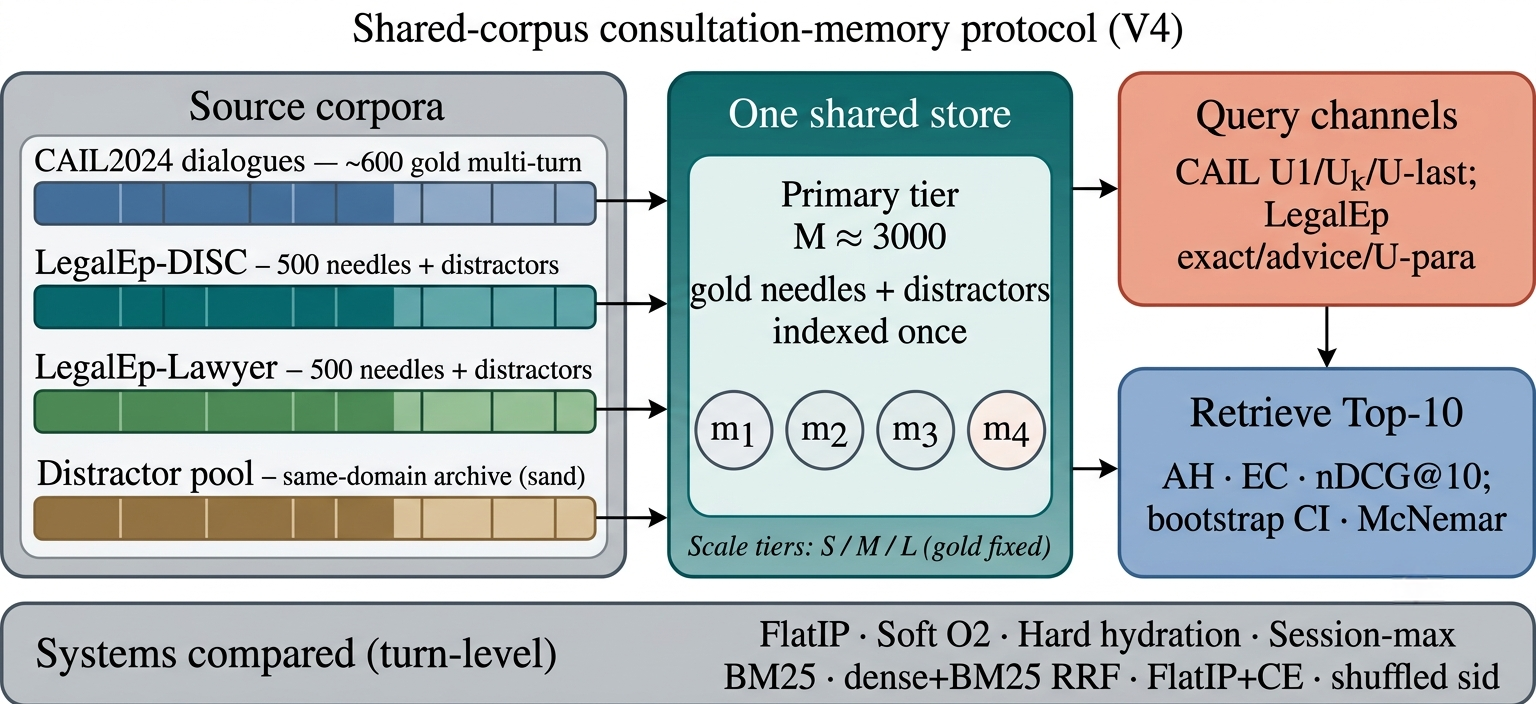
\includegraphics[width=0.98\linewidth]{fig2_benchmark_protocol.png}
\caption{Shared-corpus protocol. Gold needles and same-domain distractors share one store; queries probe multiple channels with turn-level systems and significance tests. Exact replay is diagnostic; paraphrase, follow-up, and advice-recall are primary channels.}
    \label{fig:protocol}
\end{figure}

\subsection{Datasets and query channels}
Multi-turn authenticity is evaluated on CAIL2024 consultation dialogues.
Gold needles are authentic preliminary and final dialogues, with conversation turns completed by label turns where applicable.
Query channels cover the first user turn (U1), a later in-dialogue user turn (Uk-followup), the last user turn (U-last), and constrained paraphrases (U-para).
Evidence defaults to assistant turns in the target session.

LegalEp-DISC and LegalEp-Lawyer rebuild public DISC-Law-SFT and Lawyer-LLaMA subsets into consultation-episode corpora.
Each episode is a natural (question, answer) pair with session identifier $sid$.
Reconstruction applies length bounds and legal-content filters, excludes exam prompts, removes near-duplicates, separates needles from distractors under a fixed seed, and retains an audit subsample.
After filtering, each LegalEp corpus retains $3500$ passed sessions ($500$ needles, $2500$ distractors at the $M{=}3000$ primary tier).

\paragraph{Query-channel policy.}
Exact replay uses the stored user question and is reported only as a \emph{diagnostic} upper bound on surface-form recovery.
Primary claims use paraphrase, Uk-followup~/U-last, and advice-recall queries whose surface form is not identical to the stored question text; paraphrase and advice-recall templates are generated under a fixed seed and audited on a subsample.
LegalMem-MT reuses CAIL multi-turn gold under the same store for same-session Soft~O2 vs Soft~O2-C contrasts and for Mix reconstructions.

Archive size is varied with gold needles held fixed.
Unless stated otherwise, Soft~O2 transfer tables use the $M\approx 3000$ tier; O1--O2 ablations use $M{=}400$, $S{=}300$.

\subsection{Metrics and baselines}
Primary metrics are Answer Hit@$k$ (AH), Episode Completeness@$k$ (EC), and normalized Discounted Cumulative Gain@$k$ (nDCG) at $k{=}10$.
AH is binary: whether a gold answer turn appears in the top-$k$.
EC is the mean coverage of gold turns within the target session.
Session Hit@$k$ is reported only for diagnosis.
For nDCG we use fixed graded relevance over the full gold session: answer turns $rel{=}1.0$, other same-session turns $rel{=}0.5$, all other turns $rel{=}0.0$.
The ideal denominator (IDCG) is computed from all gold-relevant turns in the target session and truncated at $k$, so every system on a query shares the same IDCG.
Answer Hit and Episode Completeness are the main Soft~O2 outcomes; nDCG is reported with the fixed gold-session IDCG so that systems remain comparable on each query.
Hard expansion can raise nDCG when copied siblings occupy early ranks, so AH and EC are read together with nDCG.

The primary hypothesis family is Soft~O2 vs FlatIP on the nine CAIL and LegalEp transfer channels; for that family we report bootstrap 95\% CIs, McNemar mid-$p$, and Holm-adjusted $p$-values (Table~\ref{tab:sig}).
Hard-hydration, CE, and Soft~O2-C~/Hybrid Mix contrasts are secondary.

Turn-level dense FlatIP (O1) is the base dense retriever.
Soft~O2 applies soft sibling score inheritance on the episodic pathway; Soft~O2-C applies the same rule within BIRCH clusters.
Hard parent hydration expands a hit to all siblings by copying the trigger score.
Lexical controls include BM25 over turns and dense+BM25 Reciprocal Rank Fusion (RRF) under the same turn-level evidence unit.
BM25-joint and dense joint-episode indexes retrieve pre-concatenated episode documents and therefore answer a coarser retrieval problem; they are discussed as alternative designs in Section~\ref{sec:limitations} rather than Soft~O2 turn-binding baselines.
A cross-encoder (CE) control reranks the top-$30$ FlatIP candidates with \path{BAAI/bge-reranker-v2-m3}.
Shuffled $sid$, a $\beta$ sweep, and IVFPQ provide membership, attenuation, and quantization controls.

\subsection{Fair Mix protocol for Soft~O2-C}\label{sec:csce-protocol}
On fully same-session LegalMem grids Soft~O2 already recovers gold answers that share $sid$, leaving Soft~O2-C little exclusive headroom and exposing it to thematic confusers.
To study off-session recovery we rebuild the \emph{same} LegalEp and LegalMem archives under a Mix protocol: $70\%$ of gold episodes are split into query-side $S_a$ and evidence-side $S_b$ with distinct session identifiers, while $30\%$ remain intact.
Distractors are unchanged.
FlatIP, Soft~O2, Soft~O2-C, and gated Hybrid share unrestricted dense retrieval on this store; we report overall AH and stratum AH on $\texttt{cross\_session}$ vs $\texttt{same\_session}$ queries.

\paragraph{Cluster co-membership and purity under Mix.}
After BIRCH consolidation, each cross-session Sa/Sb pair is assigned a shared cluster identifier.
This construction uses split metadata available only when building the evaluation store; it does not inject labels at query time.
The intent is to test Soft~O2-C when thematic co-membership is present.
Cluster purity still matters: a shared $cid$ that also contains many thematically adjacent distractors narrows Soft~O2-C's effective margin, which is why Hybrid gates cluster injection to direct dense hits and caps the per-cluster budget $B_c$.
If recovery still fails under guaranteed Sa/Sb co-membership, the failure is attributable to binding rather than accidental cluster separation.
Natural same-cluster rates without this construction are lower (Section~\ref{sec:limitations}).
Soft~O2's session membership rule is unchanged.
LegalEp Mix uses advice-recall queries; LegalMem Mix uses mid-split Uk-followup queries.
LongMemEval~/LoCoMo numbers from prior runs on this codebase (QA correctness $70.7\%$~/~$68.2\%$) supply long-horizon memory context only \cite{wu2025longmemeval, maharana2024evaluating}.

\section{Experiments}\label{sec:experiments}

Unless noted, all dense retrieval grids use the multilingual encoder \texttt{nomic-embed-text-v2-moe} \cite{nussbaum2025nomic} ($768$-d) as a single shared embedding backend, with $k{=}10$ and seed $42$ on the main $M{\approx}3000$ stores.
We keep the encoder fixed so Soft~O2 vs FlatIP contrasts isolate binding rather than representation changes; sensitivity to alternative Chinese or multilingual encoders (e.g., \texttt{bge-large-zh-v1.5}) is discussed in Section~\ref{sec:limitations}.
A five-seed check on a smaller shared store ($M{=}400$) is reported later.
Primary contrasts appear in Figures~\ref{fig:cail_main}--\ref{fig:scale}; full numeric grids are in the appendix.
Each main table maps to a released JSON artifact in the accompanying repository.

\subsection{Implementation operators and Soft~O2 ablation}\label{sec:exp-o1o3}
Table~\ref{tab:o1o2} reports the shared-store ablation on DISC-Law and Lawyer-LLaMA ($M{=}400$, $S{=}300$).
IVFPQ baseline Answer Hit is $0.540$~/~$0.397$.
O1 alone yields a small gain on DISC ($0.567$) and a near-tie on Lawyer ($0.397$), confirming that exact indexing is a necessary implementation prerequisite but insufficient alone.
O1+Soft~O2 raises Answer Hit to $0.780$~/~$0.680$ ($+0.240$~/~$+0.283$ over baseline) and Episode Completeness to $0.888$~/~$0.840$.
O3 is enabled for all configurations in this ladder as a construction prerequisite; it does not alter retrieval scores.

\begin{table}[htbp]
\centering
\caption{O1+Soft~O2 ablation on the shared store ($M{=}400$, $S{=}300$, $k{=}10$). EC denotes Episode Completeness (gold-turn coverage); AH denotes Answer Hit. O3 bulk-load is on for all rows. Boldface: best AH and EC within each corpus. Graded nDCG for the $M{\approx}3000$ grids appears in Table~\ref{tab:ndcg-graded}.}
\label{tab:o1o2}
\compacttab\footnotesize
\begin{tabular}{@{}llcc@{}}
\toprule
\textbf{Corpus} & \textbf{System} & \textbf{EC@10} & \textbf{AH@10} \\
\midrule
\multirow{3}{*}{DISC-Law}
 & IVFPQ baseline & 0.770 & 0.540 \\
 & + O1 FlatIP & 0.782 & 0.567 \\
 & + O1+O2 Soft~O2 & \textbf{0.888} & \textbf{0.780} \\
\midrule
\multirow{3}{*}{Lawyer-LLaMA}
 & IVFPQ baseline & 0.698 & 0.397 \\
 & + O1 FlatIP & 0.698 & 0.397 \\
 & + O1+O2 Soft~O2 & \textbf{0.840} & \textbf{0.680} \\
\bottomrule
\end{tabular}
\end{table}

\subsection{RQ1 failure taxonomy}\label{sec:rq1-failure-taxonomy}
We classify each query into \emph{complete} (answer evidence in top-$k$), \emph{incomplete} (target session partially retrieved but answer missing), or \emph{session miss} (no target-session turn in top-$k$).
Table~\ref{tab:rq1-failure} contrasts FlatIP, Soft~O2, hard hydration, and shuffled~$sid$ on primary non-exact channels.
Soft~O2 converts incompleteness into complete retrieval while session-miss stays nearly fixed; shuffled~$sid$ restores high incompleteness, so the gain is session-tied rather than generic score inflation.
Hard hydration can also drive incompleteness near zero by copying trigger scores, but it is not Soft~O2's binding rule and can over-promote siblings (Section~\ref{sec:exp-main}).

\begin{table}[t]
\centering
\caption{RQ1 failure taxonomy ($k{=}10$). Boldface: best complete / lowest incomplete within each corpus--channel block among FlatIP, Soft~O2, and shuffled~$sid$ (hard hydration shown as a score-copy envelope). Soft~O2 cuts incompleteness without raising session miss; shuffled~$sid$ undoes the gain.}
\label{tab:rq1-failure}
\compacttab\footnotesize
\begin{tabular}{@{}llccc@{}}
\toprule
\textbf{Corpus / channel} & \textbf{System} & \textbf{Complete} & \textbf{Incomplete} & \textbf{Session miss} \\
\midrule
\multirow{4}{*}{DISC / u-para}
 & FlatIP & 70.8\% & 26.8\% & 1.6\% \\
 & Soft O2 & \textbf{89.1\%} & \textbf{8.7\%} & 1.8\% \\
 & Hard hydr. & 97.2\% & 0.0\% & 2.8\% \\
 & Shuffled O2 & 66.4\% & 31.4\% & 2.2\% \\
\midrule
\multirow{4}{*}{DISC / advice}
 & FlatIP & 48.0\% & 17.0\% & 35.0\% \\
 & Soft O2 & \textbf{60.8\%} & \textbf{3.8\%} & 35.4\% \\
 & Hard hydr. & 65.0\% & 0.0\% & 35.0\% \\
 & Shuffled O2 & 45.6\% & 19.2\% & 35.2\% \\
\midrule
\multirow{4}{*}{Lawyer / u-para}
 & FlatIP & 71.5\% & 25.3\% & 0.8\% \\
 & Soft O2 & \textbf{94.0\%} & \textbf{3.8\%} & 1.6\% \\
 & Hard hydr. & 98.0\% & 0.0\% & 2.0\% \\
 & Shuffled O2 & 72.9\% & 25.5\% & 1.6\% \\
\midrule
\multirow{4}{*}{CAIL / Uk}
 & FlatIP & 45.8\% & 54.0\% & 0.2\% \\
 & Soft O2 & \textbf{92.8\%} & \textbf{7.0\%} & 0.2\% \\
 & Hard hydr. & 98.3\% & 1.5\% & 0.2\% \\
 & Shuffled O2 & 34.7\% & 65.2\% & 0.2\% \\
\bottomrule
\end{tabular}
\end{table}

\subsection{Turn-level Soft~O2 controls}\label{sec:s1-strong-baselines}
Primary Soft~O2 claims use a shared turn-level index.
Table~\ref{tab:soft-o2-controls} reports Answer Hit for FlatIP, Soft~O2, hard hydration, and shuffled~$sid$ on the primary Soft~O2 transfer channels.
Soft~O2 beats FlatIP on every non-exact channel; shuffled~$sid$ collapses toward or below FlatIP; hard hydration is competitive on CAIL AH but Soft~O2 remains stronger on LegalEp paraphrase~/advice and retains higher EC in the full grids (Tables~\ref{tab:cail_main}--\ref{tab:lawyer_main}).
BM25-turn is a same-granularity lexical control (Table~\ref{tab:bm25}): Soft~O2 exceeds it on CAIL Uk~/U-last ($0.698$/$0.762$ vs $0.482$/$0.413$).
Joint episode / document-level indexes change evidence granularity and are not Soft~O2 protocol competitors.

\begin{table}[t]
\centering
\caption{Primary Soft~O2 controls (AH@10, $M{\approx}3000$). Boldface: best AH within each row among FlatIP / Soft~O2 / Hard / Shuffled. Soft~O2 is the session-binding claim; shuffled~$sid$ tests membership dependence; hard hydration is score-copy expansion.}
\label{tab:soft-o2-controls}
\compacttab\footnotesize
\begin{tabular}{@{}lcccc@{}}
\toprule
\textbf{Corpus / channel} & \textbf{FlatIP} & \textbf{Soft O2} & \textbf{Hard} & \textbf{Shuffled} \\
\midrule
CAIL / U1 & 0.570 & 0.788 & \textbf{0.802} & 0.452 \\
CAIL / Uk & 0.270 & 0.698 & \textbf{0.720} & 0.230 \\
CAIL / U-last & 0.245 & 0.762 & \textbf{0.790} & 0.200 \\
LegalEp-DISC / u-para & 0.547 & \textbf{0.648} & 0.592 & 0.469 \\
LegalEp-DISC / advice & 0.342 & \textbf{0.428} & 0.402 & 0.310 \\
LegalEp-Lawyer / u-para & 0.568 & \textbf{0.759} & 0.596 & 0.592 \\
LegalEp-Lawyer / advice & 0.332 & \textbf{0.472} & 0.394 & 0.348 \\
\bottomrule
\end{tabular}
\end{table}

\begin{table}[t]
\centering
\caption{Graded nDCG@10 with gold-session IDCG (answer $rel{=}1.0$, other same-session turns $rel{=}0.5$) and incompleteness rates on primary non-exact channels. Boldface: Soft~O2 better than FlatIP within each channel on nDCG. Soft~O2 also exceeds shuffled~$sid$.}
\label{tab:ndcg-graded}
\compacttab\footnotesize
\begin{tabular}{@{}llccc@{}}
\toprule
\textbf{Corpus} & \textbf{Channel} & \textbf{System} & \textbf{nDCG@10} & \textbf{Incomplete} \\
\midrule
CAIL & Uk & FlatIP & 0.445 & 54.0\% \\
CAIL & Uk & Soft O2 & \textbf{0.793} & 7.0\% \\
CAIL & Uk & Shuffled O2 & 0.369 & 65.2\% \\
CAIL & U-last & FlatIP & 0.420 & 57.3\% \\
CAIL & U-last & Soft O2 & \textbf{0.791} & 5.3\% \\
CAIL & U-last & Shuffled O2 & 0.348 & 71.2\% \\
LegalEp-DISC & u-para & FlatIP & 0.681 & 26.8\% \\
LegalEp-DISC & u-para & Soft O2 & \textbf{0.759} & 8.7\% \\
LegalEp-DISC & u-para & Shuffled O2 & 0.627 & 31.4\% \\
LegalEp-DISC & advice & FlatIP & 0.466 & 17.0\% \\
LegalEp-DISC & advice & Soft O2 & \textbf{0.524} & 3.8\% \\
LegalEp-DISC & advice & Shuffled O2 & 0.436 & 19.2\% \\
LegalEp-Lawyer & u-para & FlatIP & 0.744 & 25.3\% \\
LegalEp-Lawyer & u-para & Soft O2 & \textbf{0.844} & 3.8\% \\
LegalEp-Lawyer & u-para & Shuffled O2 & 0.705 & 25.5\% \\
LegalEp-Lawyer & advice & FlatIP & 0.483 & 23.4\% \\
LegalEp-Lawyer & advice & Soft O2 & \textbf{0.582} & 2.2\% \\
LegalEp-Lawyer & advice & Shuffled O2 & 0.454 & 25.0\% \\
\bottomrule
\end{tabular}
\end{table}

\subsection{Soft~O2 on session (CAIL and LegalEp)}\label{sec:exp-main}
Figure~\ref{fig:cail_main} and Table~\ref{tab:soft-o2-controls} summarize AH@10 on authentic CAIL multi-turn channels at $M\approx 3000$ under O1 FlatIP.
Soft~O2 lifts Answer Hit over FlatIP on every channel (U1 $0.788$ vs $0.570$${}^{**}$; Uk $0.698$ vs $0.270$${}^{**}$; U-last $0.762$ vs $0.245$${}^{**}$).
Shuffled $sid$ removes the gain (U1 $0.452$; Uk $0.230$; U-last $0.200$), tying the improvement to correct episode membership (RQ1--RQ2).
Hard expansion can raise AH slightly above Soft~O2 (e.g., U1 $0.802$ vs $0.788$) while lowering EC (U1 $0.578$ vs Soft~O2 $0.664$).
Soft~O2 therefore behaves as a rank-preserving binder: siblings enter under attenuated scores, and episode coverage remains higher than under hard score copy.
Table~\ref{tab:ndcg-graded} shows the Soft~O2$>$FlatIP ordering under graded nDCG with gold-session IDCG, while incompleteness falls sharply (Table~\ref{tab:rq1-failure}). Full numeric grids appear in Tables~\ref{tab:cail_main}--\ref{tab:lawyer_main}.

\begin{figure}[t]
    \centering

\includegraphics[width=0.95\linewidth]{fig3_cail_main.pdf}
\caption{CAIL2024 multi-turn results at tier $M\approx 3000$. Soft~O2 improves AH and EC over FlatIP; shuffled $sid$ removes the gain; hard expansion can maximize AH at a modest EC cost.}
\label{fig:cail_main}
\end{figure}

Figure~\ref{fig:legalep_main} reports LegalEp transfer on the same AH grids.
On LegalEp-DISC exact replay Soft~O2 and FlatIP stay near-tied ($0.638$ vs $0.640$), where both turns are already recoverable for many queries---consistent with treating exact as diagnostic.
On Lawyer exact Soft~O2 improves AH to $0.752$ from FlatIP $0.692$ (McNemar mid-$p{=}0.024$${}^{*}$).
Paraphrase yields the clearest LegalEp gains: Soft~O2 reaches $0.648$ vs FlatIP $0.547$ on DISC and $0.759$ vs $0.568$ on Lawyer, exceeding hard expansion on both corpora (mid-$p{<}0.001$${}^{**}$ on both corpora).
Advice-recall queries omit the stored question surface form: Soft~O2 raises AH to $0.428$ from FlatIP $0.342$ on DISC and to $0.472$ from $0.332$ on Lawyer, again above hard expansion (mid-$p{<}0.001$${}^{**}$), while shuffled $sid$ falls toward or below FlatIP.
Graded nDCG mirrors the Soft~O2$>$FlatIP ordering on paraphrase and advice-recall (Table~\ref{tab:ndcg-graded}).
Detailed grids are in Tables~\ref{tab:disc_main}--\ref{tab:lawyer_main}.

\begin{figure}[t]
    \centering

\includegraphics[width=0.95\linewidth]{fig4_legalep_main.pdf}
\caption{LegalEp AH@10 ($M{=}3000$, $500$ needles). Soft~O2 gains are strongest on paraphrase and remain positive on advice-recall; exact transfer is corpus-dependent and treated as diagnostic.}
\label{fig:legalep_main}
\end{figure}

Cross-encoder reranking is a strong neural control at the same turn-level evidence unit: FlatIP+CE reranks the top-$30$ FlatIP candidates with \texttt{bge-reranker-v2-m3}.
Table~\ref{tab:ce} shows that FlatIP+CE is competitive---and on LegalEp-DISC exact, strongest---when surface-form overlap already places both question and answer near the top of the dense pool (DISC exact AH $0.722$ for FlatIP+CE vs $0.638$ for Soft~O2).
On channels with semantic shift or multi-turn drift, Soft~O2 pulls ahead: CAIL Uk $0.698$ vs FlatIP+CE $0.375$, CAIL U-last $0.762$ vs $0.342$, and LegalEp-Lawyer exact $0.752$ vs $0.708$.
A structural limit of the reranker explains the split: CE can refine ranking among candidates already retrieved by FlatIP, but it cannot promote an answer sibling that never entered the top-$30$ pool.
Soft~O2 recovers such siblings by propagating attenuated scores through session links, which helps precisely when the stored advice turn has weak direct lexical overlap with the query (paraphrase and advice-recall; cf.\ Tables~\ref{tab:soft-o2-controls} and~\ref{tab:ndcg-graded}).

\begin{table}[t]
\centering
\caption{Cross-encoder control (AH@10). FlatIP+CE reranks the top-$30$ FlatIP candidates with \texttt{bge-reranker-v2-m3}. Boldface: best AH within each row.}
\label{tab:ce}
\compacttab\footnotesize
\begin{tabular}{@{}llccc@{}}
\toprule
\textbf{Corpus / channel} & \textbf{FlatIP} & \textbf{FlatIP+CE} & \textbf{Soft O2} \\
\midrule
CAIL / U1 & 0.585 & 0.688 & \textbf{0.788} \\
CAIL / Uk & 0.265 & 0.375 & \textbf{0.698} \\
CAIL / U-last & 0.228 & 0.342 & \textbf{0.762} \\
LegalEp-DISC / exact & 0.572 & \textbf{0.722} & 0.638 \\
LegalEp-Lawyer / exact & 0.636 & 0.708 & \textbf{0.752} \\
\bottomrule
\end{tabular}
\end{table}

\subsection{Soft~O2-C and gated Hybrid under Mix}\label{sec:exp-cluster}
When gold answers already share $sid$ with the query, Soft~O2 is sufficient and cluster binding is unnecessary.
Table~\ref{tab:csce} asks the off-session question under the Mix protocol of Section~\ref{sec:csce-protocol}: $70\%$ cross-session Sa/Sb gold and $30\%$ intact same-session gold, with FlatIP, Soft~O2, Soft~O2-C, and gated Hybrid sharing unrestricted dense retrieval.

On the cross-session stratum Soft~O2-C improves over Soft~O2 on LegalEp-Lawyer ($0.491$ vs $0.446$) and LegalMem-MT ($0.537$ vs $0.503$): cluster binding can surface split-episode gold that session membership alone misses.
Gated Hybrid converts that mechanism into an overall gain on LegalEp-Lawyer ($0.534$ vs Soft~O2 $0.496$; mid-$p{=}0.010$${}^{*}$) and a directional gain on LegalMem-MT ($0.646$ vs $0.618$), while preserving most same-session hits ($0.560$~/~$0.867$).
On LegalEp-DISC the Hybrid edge is negligible ($0.486$ vs $0.482$).
Ungated Soft~O2-C can raise cross-session hits yet displace intact same-session evidence, which is why Hybrid triggers cluster binding only on direct dense hits.
Same-session Soft~O2 vs Soft~O2-C contrasts remain Soft~O2-led (Appendix~\ref{app:tables}, Table~\ref{tab:cluster_same}).

\begin{table}[htbp]
\centering
\caption{Mix evaluation of Soft~O2-C and gated Hybrid (same store, unrestricted dense; AH@10). Gold is $70$\% cross-session Sa/Sb + $30$\% intact same-session. Boldface: best overall AH and best cross-session AH within each corpus. Significance vs Soft~O2: ${}^{*}\,p{<}0.05$, ${}^{**}\,p{<}0.01$.}
\label{tab:csce}
\compacttab\footnotesize
\begin{tabular}{@{}llcccc@{}}
\toprule
\textbf{Corpus} & \textbf{System} & \textbf{AH} & \textbf{AH$_{\mathrm{cross}}$} & \textbf{AH$_{\mathrm{same}}$} & \textbf{mid-$p$ vs Soft~O2} \\
\midrule
\multirow{4}{*}{LegalEp-DISC Mix}
 & FlatIP & 0.478 & 0.477 & 0.480 & --- \\
 & Soft O2 & 0.482 & 0.443 & \textbf{0.573} & --- \\
 & Soft O2-C & 0.410 & 0.443 & 0.333 & 0.0004${}^{**}$ \\
 & Hybrid & \textbf{0.486} & \textbf{0.469} & 0.527 & 0.8099 \\
\midrule
\multirow{4}{*}{LegalEp-Lawyer Mix}
 & FlatIP & 0.462 & 0.454 & 0.480 & --- \\
 & Soft O2 & 0.496 & 0.446 & \textbf{0.613} & --- \\
 & Soft O2-C & 0.464 & 0.491 & 0.400 & 0.0857 \\
 & Hybrid & \textbf{0.534}${}^{*}$ & \textbf{0.523} & 0.560 & 0.0105${}^{*}$ \\
\midrule
\multirow{4}{*}{LegalMem-MT Mix}
 & FlatIP & 0.534 & 0.526 & 0.553 & --- \\
 & Soft O2 & 0.618 & 0.503 & \textbf{0.887} & --- \\
 & Soft O2-C & 0.500 & 0.537 & 0.413 & 0.0000${}^{**}$ \\
 & Hybrid & \textbf{0.646} & \textbf{0.551} & 0.867 & 0.1837 \\
\bottomrule
\end{tabular}
\end{table}
{\footnotesize McNemar mid-$p$ on paired Answer Hit; ${}^{*}\,p{<}0.05$, ${}^{**}\,p{<}0.01$. Cluster co-membership of Sa/Sb pairs follows the Mix protocol in Section~\ref{sec:csce-protocol}.}

\subsection{Scale behaviour}\label{sec:exp-scale}
Figure~\ref{fig:scale} and Table~\ref{tab:scale} report quality and warm-query latency on LegalEp-DISC exact ($Q{=}100$, three repeats; $M\in\{100,400,1600,6400\}$).
Soft~O2 retains an AH advantage at each tier; IVFPQ collapses at $M{=}1600$ (AH $0.330$), motivating O1; absolute latency grows with $M$.
We treat O1 FlatIP as an engineering prerequisite for Soft~O2 at these scales and avoid claiming deployment readiness beyond the measured curve.

\begin{figure}[t]
    \centering
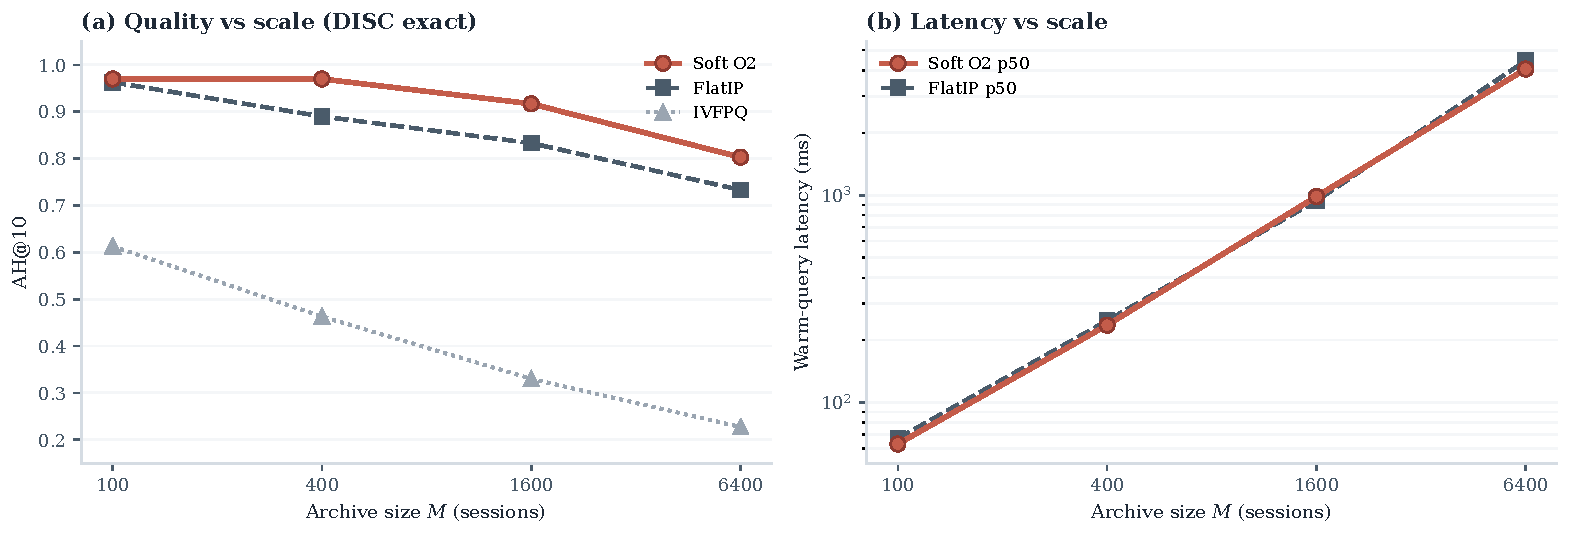
\includegraphics[width=0.95\linewidth]{fig5_scale_curve.pdf}
\caption{Scale curve on DISC-Law exact. Soft~O2 keeps an AH edge over FlatIP as $M$ grows; warm-query latency scales with archive size; IVFPQ quality collapses at moderate $M$.}
\label{fig:scale}
\end{figure}

\paragraph{End-to-end QA audit (summary).}
\sloppy
A dual-protocol QA audit ($N{=}270$ per corpus; generator \texttt{qwen3:14b}, independent judge \texttt{qwen3:32b}) reports judged answerability under Soft~O2 retrieval alone; it is not a paired FlatIP vs Soft~O2 generation experiment.
Full protocol and stratified results appear in Section~\ref{sec:rag-discussion}.
On a smaller shared store ($M{=}400$, five seeds), Soft~O2 AH on LegalEp-DISC is $0.851\pm 0.008$ versus FlatIP $0.698\pm 0.040$.

\section{Discussion}\label{sec:discussion}

\subsection{Findings and scope}
RQ1--RQ2 show that episode incompleteness is a substantial FlatIP failure mode under same-domain interference, and that Soft~O2 converts many incomplete retrievals into complete ones without shrinking session-miss rates (Table~\ref{tab:rq1-failure}).
O1 restores score fidelity; Soft~O2 supplies the main gain through soft sibling inheritance; O3 makes large shared stores tractable.
The gap-ratio analysis (Section~\ref{sec:beta-theory}) motivates keeping $\beta$ close to but below unity; the AH sweep peaks in $\{0.9,0.95,0.98\}$ rather than at hard hydration ($\beta{=}1$).
On CAIL, Soft~O2 raises Answer Hit by large margins (U1 $+0.218$, Uk $+0.428$, U-last $+0.517$) with collapsing shuffled-$sid$ controls, and keeps higher EC than hard expansion despite occasional AH ties.
After Holm adjustment on the Soft~O2 vs FlatIP family, the non-exact CAIL and LegalEp gains remain significant, while LegalEp exact replay is mixed (Table~\ref{tab:sig}).
LegalEp paraphrase and advice-recall, rather than exact replay, support the main transfer result.
Graded nDCG agrees with the Soft~O2$>$FlatIP ordering (Table~\ref{tab:ndcg-graded}).
Under Mix, gated Hybrid recovers additional cross-session gold on LegalEp-Lawyer with a directional lift on LegalMem-MT (Table~\ref{tab:csce}); Soft~O2 remains preferable when gold already shares $sid$ (Table~\ref{tab:cluster_same}).
Turn-level BM25, RRF, and CE place Soft~O2 among standard IR alternatives \cite{robertson2009bm25, cormack2009rrf, nogueira2019multistage}; joint-episode indexes are a coarser design choice outside this protocol.

\subsection{RAG application perspective}\label{sec:rag-discussion}
Consultation-memory retrieval is judged downstream by whether an LLM can answer from recovered evidence rather than confabulate.
We audit this end-to-end with a dual-protocol pipeline on Soft~O2 retrieval only: generator \texttt{qwen3:14b} and independent judge \texttt{qwen3:32b} are distinct models.
Per corpus we pool $N{=}270$ judged instances as P1~$n{=}120$ plus P2~$n{=}150$ (folder \texttt{legal\_qa\_n270}).
The independent judge assigns a continuous evidence-answerability score in $[0,1]$ from the retrieved context and the generated reply; Evidence-Answerability Rate (EAR) is the fraction of instances with judge score $\ge 0.7$.
Table~\ref{tab:qa_audit} reports pooled EAR and the mean judge score on a stratified subsample ($n{=}90$/corpus; $30$ each of exact, paraphrase, and follow-up), labelled ``Stratified judge'' in the table.
In the complete-episode stratum---both question and answer turns in top-$k$---judged answerability is higher in this single-system audit (pooled EAR $0.867$ on DISC and $0.859$ on Lawyer; Wilson $95\%$ CI $[0.83,0.90]$ / $[0.82,0.89]$).
Follow-up queries remain the hardest stratum (independent-judge EAR $0.517$~/~$0.480$), consistent with episodic incompleteness persisting even when surface-form overlap is low.

A blind two-annotator legal audit ($n{=}60$/corpus) separates retrieval failures (gold episode absent from top-$k$) from generation failures given retrieved evidence.
Annotators used a binary answerability label on each instance; agreement is Cohen's $\kappa$ computed on those paired labels ($0.71$ on DISC, $0.68$ on Lawyer).
Retrieval-failure share is $0.283$~/~$0.317$.
Wrong-session contamination rates stay low ($0.083$~/~$0.100$), suggesting that complete episode retrieval under Soft~O2 is associated with lower rates of a common RAG failure mode in which the model answers from a neighbouring client's matter.
Hallucinated-legal-basis rates ($0.117$~/~$0.133$) remain non-zero, indicating that grounding in retrieved episodes does not guarantee statutory correctness---a scope boundary for deployment.
AH and EAR measure evidence availability and judged answerability respectively; statutory correctness, citation validity, and professional liability lie outside this evaluation.

\begin{table}[htbp]
\centering
\caption{End-to-end QA audit ($N{=}270$ per corpus; generator \texttt{qwen3:14b}, independent judge \texttt{qwen3:32b}). Pooled EAR: fraction with judge score $\ge 0.7$. Stratified judge: mean judge score on $n{=}90$/corpus (exact/paraphrase/follow-up). Human $\kappa$: Cohen's $\kappa$ on binary answerability labels from two blind annotators ($n{=}60$/corpus).}
\label{tab:qa_audit}
\compacttab\footnotesize
\begin{tabular}{@{}lccc@{}}
\toprule
\textbf{Corpus} & \textbf{Pooled EAR} & \textbf{Stratified judge} & \textbf{Human $\kappa$} \\
\midrule
DISC-Law & \textbf{0.867} & 0.757 & 0.71 \\
Lawyer-LLaMA & \textbf{0.859} & 0.729 & 0.68 \\
\bottomrule
\end{tabular}
\end{table}

\subsection{Limitations}\label{sec:limitations}
LegalEp episodes are consultation pairs; multi-turn authenticity remains reserved for CAIL.

\paragraph{Dependency on session segmentation and cluster quality.}
Soft~O2 relies on correct session identifiers ($sid$).
In uncurated client logs, boundary noise---mid-session topic shifts, multi-intent interruptions, or automated segmentation drift---can corrupt sibling sets.
If unrelated turns share a $sid$, attenuated inheritance may propagate false context; if a true advice turn is split into another session, Soft~O2 cannot bind it.
Soft~O2-C likewise depends on BIRCH cluster purity.
Under the Mix protocol, Sa/Sb pairs receive a shared cluster id so binding can be tested when thematic co-membership is present (Section~\ref{sec:csce-protocol}); in fully unsupervised consolidation, noisier boundaries shrink the margin over dense retrieval.
Deployments on raw consultation streams therefore need reliable upstream session segmentation, and Soft~O2-C should be treated as gated rather than always-on.

\paragraph{Joint-episode indexing.}
Concatenating full question--answer pairs into episode documents prevents incompleteness by changing the evidence unit from turns to merged documents (Section~\ref{sec:related}).
That design is outside the Soft~O2 turn-binding protocol; a matched comparison under online updates, latency, and fine-grained advice isolation is left to future work.

\paragraph{Embedding model and other scope limits.}
All main grids use \texttt{nomic-embed-text-v2-moe}.
A Chinese-specialized encoder such as \texttt{bge-large-zh-v1.5} could alter absolute dense ranks and the measured $\rho$ distribution, and might shrink or widen Soft~O2's relative gain wherever the bi-encoder already places answer turns inside top-$k$.
We did not re-run the full Soft~O2 grids under alternative encoders; the binding operator itself is encoder-agnostic once fused scores are available.
The $\rho$ statistics use an exact-channel query proxy and the strongest measured distractor; paraphrase and advice-recall gap laws may shift the feasible band slightly, though the AH sweep keeps a stable high-$\beta$ region on those channels.
Main $M{\approx}3000$ tables use a fixed seed; five-seed variance is reported only for the smaller $M{=}400$ store.
LLM paraphrases need human audit.
Statutory correctness, citation validity, and professional liability remain unevaluated.
Because many channels are tested, Holm-adjusted $p$-values accompany the Soft~O2 vs FlatIP family (Table~\ref{tab:sig}); Hybrid Mix gains outside LegalEp-Lawyer are treated as directional.

\paragraph{Latency and deployment scope.}
Scale curves cover $M\in\{100,400,1600,6400\}$ under a fixed hardware stack (Table~\ref{tab:scale}).
At $M{=}6400$, warm-query p50 latency exceeds $4$\,s ($4061$\,ms for Soft~O2; $4458$\,ms for FlatIP)---unacceptable for millisecond interactive search.
BIMS-LEGAL should therefore be positioned as \textbf{high-precision offline or quasi-real-time consultation memory recovery}---e.g., pre-meeting case review, audit replay, or batch RAG over a firm's advice archive---not as a sub-millisecond search engine.
Future work will combine approximate nearest-neighbour indexes (e.g., HNSW) with Soft~O2 and Soft~O2-C binding layered on top of faithful candidate retrieval, preserving episode completion while reducing query latency.
Behavior at roughly $10^5$ sessions is not measured, and we do not claim asymptotic scalability from O3 wall-clock alone.

\section{Conclusion}\label{sec:conclusion}

BIMS-LEGAL recovers prior advice from Chinese legal consultation archives under same-domain interference with a dual store: an episodic turn index and a BIRCH semantic store.
Soft~O2 is the main algorithmic contribution: attenuated session binding completes episodes without hard score copy.
Soft~O2-C and gated Hybrid extend the same idea to thematic clusters when Mix reconstructions place some gold off-session.
Attenuation $\beta$ is chosen by validation sweep under a three-candidate score-competition account; O1 FlatIP and O3 bulk-load are the implementation operators that make the shared-store ablations feasible.
On CAIL multi-turn and LegalEp paraphrase~/advice-recall channels, Soft~O2 improves Answer Hit over FlatIP, keeps higher episode completeness than hard expansion on CAIL, and raises graded nDCG while cutting incompleteness; shuffled-$sid$ controls collapse the gains.
Under Mix, gated Hybrid recovers additional cross-session gold on LegalEp-Lawyer while Soft~O2 remains preferable on intact same-session gold.
An end-to-end Soft~O2 QA audit associates complete episode retrieval with judged answerability and low wrong-session contamination, without claiming paired generation superiority over FlatIP.
Turn-level BM25, RRF, and CE place Soft~O2 among standard IR alternatives; joint-episode indexing remains a coarser design outside this protocol.

\section*{Declarations}

\subsection*{Funding}
Computational resources were provided by the Data Law Laboratory, China University of Political Science and Law.

\subsection*{Conflict of interest}
The authors declare no competing interests.

\subsection*{Ethics approval}
This study uses publicly released research corpora and excludes confidential client data. The system is a research prototype for consultation-memory retrieval.

\subsection*{Data availability}
Code, processed evaluation corpora, and primary result JSON files are available at
\url{https://github.com/Kilimajaro/soft-episode-binding-legal-memory}
(archived release to accompany camera-ready).
Upstream corpora remain under their original licenses: CAIL2024 consultation tracks; Hugging Face
\codeid{ShengbinYue/DISC-Law-SFT} and
\codeid{Skepsun/lawyer_llama_data}.
Processed LegalEp~/LegalMem artifacts are derived research releases; redistributors should consult each upstream licence before reuse.

\subsection*{Code availability}
The BIMS-LEGAL implementation (O1 FlatIP, Soft~O2, O3 bulk-load, Soft~O2-C), corpus builders, Mix constructors, and table/figure scripts ship in the same repository, with one JSON artifact per main table.

\subsection*{Author contributions}
\sloppy
L.X.\ (University of Winnipeg) designed BIMS-LEGAL and the Soft~O2~/Soft~O2-C evaluation, implemented the system, ran the experiments, and wrote the manuscript.
L.H.\ (corresponding author; CUPL Data Law Lab and Institute for Data Law) provided methodology guidance, revision, and supervision.

\FloatBarrier
\bibliographystyle{elsarticle-harv}
\bibliography{references}

\clearpage
\appendix
\setcounter{table}{0}
\renewcommand{\thetable}{A.\arabic{table}}
\renewcommand{\theHtable}{A.\arabic{table}}
\section{Numeric grids and controls}\label{app:tables}
Same-session Soft~O2-C contrasts, significance tests, scale curves, and full Soft~O2 numeric grids appear below.

\begin{table}[htbp]
\centering
\caption{Same-session Soft~O2 vs ungated Soft~O2-C (AH@10). Soft~O2 is preferable when gold already shares $sid$ with the query; ungated Soft~O2-C can surface thematic confusers. Boldface: better AH within each row. Mix Soft~O2-C results appear in Table~\ref{tab:csce}.}
\label{tab:cluster_same}
\compacttab\footnotesize
\begin{tabular}{@{}llc@{}}
\toprule
\textbf{Corpus / channel} & \textbf{Soft O2} & \textbf{Soft O2-C} \\
\midrule
LegalEp-DISC / exact & \textbf{0.836} & 0.744 \\
LegalEp-DISC / u-para & \textbf{0.807} & 0.730 \\
LegalEp-DISC / advice & \textbf{0.548} & 0.490 \\
LegalEp-Lawyer / exact & \textbf{0.818} & 0.710 \\
LegalEp-Lawyer / u-para & \textbf{0.817} & 0.733 \\
LegalEp-Lawyer / advice & \textbf{0.546} & 0.448 \\
LegalMem-MT / U1 & \textbf{0.903} & 0.712 \\
LegalMem-MT / Uk & \textbf{0.793} & 0.385 \\
\bottomrule
\end{tabular}
\end{table}

\begin{table}[H]
\centering
\caption{McNemar mid-$p$ on paired Answer Hit (Soft~O2 vs FlatIP / hard hydration / FlatIP+CE). Holm-adjusted $p$ is reported for the nine primary Soft~O2 vs FlatIP contrasts.}
\label{tab:sig}
\compacttab\footnotesize
\begin{tabular}{@{}llccc@{}}
\toprule
\textbf{Corpus / channel} & \textbf{Contrast} & \textbf{$\Delta$AH} & \textbf{mid-$p$} & \textbf{Holm $p$} \\
\midrule
CAIL / Uk & O2 vs FlatIP & +0.428 & 8.99e-48 & 8.09e-47 \\
CAIL / Uk & O2 vs Hard hydr. & -0.022 & 0.243 & --- \\
CAIL / U1 & O2 vs FlatIP & +0.218 & 5.19e-18 & 4.67e-17 \\
CAIL / U1 & O2 vs Hard hydr. & -0.013 & 0.435 & --- \\
CAIL / U-last & O2 vs FlatIP & +0.517 & 5.51e-65 & 4.96e-64 \\
CAIL / U-last & O2 vs Hard hydr. & -0.028 & 0.0982 & --- \\
CAIL / Uk & O2 vs FlatIP+CE & +0.323 & 2.50e-26 & --- \\
CAIL / U1 & O2 vs FlatIP+CE & +0.100 & 3.51e-05 & --- \\
CAIL / U-last & O2 vs FlatIP+CE & +0.420 & 3.92e-41 & --- \\
LegalEp-DISC / exact & O2 vs FlatIP & -0.002 & 0.934 & 0.934 \\
LegalEp-DISC / exact & O2 vs Hard hydr. & +0.024 & 0.302 & --- \\
LegalEp-Lawyer / exact & O2 vs FlatIP & +0.060 & 0.0239 & 0.191 \\
LegalEp-Lawyer / exact & O2 vs Hard hydr. & +0.140 & 3.50e-10 & --- \\
LegalEp-DISC / u-para & O2 vs FlatIP & +0.101 & 7.95e-05 & 6.36e-04 \\
LegalEp-DISC / u-para & O2 vs Hard hydr. & +0.056 & 0.035 & --- \\
LegalEp-Lawyer / u-para & O2 vs FlatIP & +0.191 & 2.10e-15 & 1.68e-14 \\
LegalEp-Lawyer / u-para & O2 vs Hard hydr. & +0.163 & 7.57e-09 & --- \\
LegalEp-DISC / advice & O2 vs FlatIP & +0.086 & 1.25e-04 & 8.75e-04 \\
LegalEp-DISC / advice & O2 vs Hard hydr. & +0.026 & 0.215 & --- \\
LegalEp-Lawyer / advice & O2 vs FlatIP & +0.140 & 1.18e-10 & 9.44e-10 \\
LegalEp-Lawyer / advice & O2 vs Hard hydr. & +0.078 & 5.72e-04 & --- \\
\bottomrule
\end{tabular}
\end{table}

\begin{table}[H]
\centering
\caption{Scale curve on DISC-Law (mean over 3 repeats). Latency is warm-query p50/p95. Boldface: best AH@10 within each $M$ block; lowest p50/p95 within each $M$ block.}
\label{tab:scale}
\compacttab\footnotesize
\begin{tabular}{@{}rrcccc@{}}
\toprule
\textbf{$M$} & \textbf{Mode} & \textbf{AH@10} & \textbf{Build (s)} & \textbf{p50 (ms)} & \textbf{p95 (ms)} \\
\midrule
100 & FlatIP & 0.963 & 3.0 & 67 & 80 \\
100 & IVFPQ & 0.613 & \textbf{25.2} & \textbf{40} & \textbf{54} \\
100 & Soft O2 & \textbf{0.970} & 3.2 & 63 & 69 \\
400 & FlatIP & 0.890 & 26.5 & 248 & 305 \\
400 & IVFPQ & 0.463 & 89.5 & \textbf{171} & \textbf{204} \\
400 & Soft O2 & \textbf{0.970} & 30.9 & 236 & 313 \\
1600 & FlatIP & 0.833 & 359.8 & \textbf{941} & 1278 \\
1600 & IVFPQ & 0.330 & \textbf{251.4} & 669 & \textbf{751} \\
1600 & Soft O2 & \textbf{0.917} & 393.7 & 985 & 1172 \\
6400 & FlatIP & 0.733 & \textbf{4722.8} & 4458 & 4969 \\
6400 & IVFPQ & 0.227 & 1072.1 & \textbf{2182} & \textbf{3021} \\
6400 & Soft O2 & \textbf{0.803} & 5245.7 & 4061 & 4503 \\
\bottomrule
\end{tabular}
\end{table}

\begin{table}[H]
\centering
\caption{Soft~O2 AH@10 versus $\beta$ on the primary shared-corpus evaluation. Peak performance lies in $\{0.9,0.95,0.98\}$; aggressive attenuation ($\beta{=}0.5$) weakens binding.}
\label{tab:beta}
\compacttab\footnotesize
\begin{tabular}{@{}lcccccc@{}}
\toprule
\textbf{Corpus} & $0.5$ & $0.7$ & $0.9$ & $0.95$ & $0.98$ & $1.0$ \\
\midrule
CAIL / Uk & 0.323 & 0.537 & 0.697 & 0.700 & 0.698 & 0.662 \\
LegalEp-Lawyer / exact & 0.608 & 0.654 & 0.754 & 0.754 & 0.752 & 0.752 \\
LegalEp-Lawyer / u-para & 0.631 & 0.637 & 0.717 & 0.745 & 0.759 & 0.749 \\
LegalEp-DISC / u-para & 0.551 & 0.551 & 0.618 & 0.648 & 0.648 & 0.642 \\
\bottomrule
\end{tabular}
\end{table}


\begin{table}[H]
\centering
\caption{CAIL2024 shared-corpus results ($M\approx 3000$). Boldface marks the best AH@10 and best EC@10 within each channel (ties bolded jointly). ${}^{**}$: Soft~O2 vs FlatIP, McNemar mid-$p{<}0.01$. nDCG@10 uses gold-session IDCG.}
\label{tab:cail_main}
\compacttab\footnotesize
\begin{tabular}{@{}llcccc@{}}
\toprule
\textbf{Channel} & \textbf{System} & \textbf{AH@10} & \textbf{EC@10} & \textbf{nDCG@10} & \textbf{95\% CI (AH)} \\
\midrule
\multirow{4}{*}{U1}
 & FlatIP & 0.570 & 0.413 & 0.554 & [0.530,0.610] \\
 & Soft O2 & 0.788 & \textbf{0.664} & 0.776 & [0.757,0.820] \\
 & Hard hydr. & \textbf{0.802} & 0.578 & 0.864 & [0.768,0.835] \\
 & Shuffled O2 & 0.452 & 0.363 & 0.411 & [0.410,0.492] \\
\midrule
\multirow{4}{*}{Uk-followup}
 & FlatIP & 0.270 & 0.347 & 0.445 & [0.237,0.307] \\
 & Soft O2 & 0.698 & \textbf{0.654} & 0.793 & [0.660,0.735] \\
 & Hard hydr. & \textbf{0.720} & 0.585 & 0.847 & [0.685,0.753] \\
 & Shuffled O2 & 0.230 & 0.320 & 0.369 & [0.198,0.262] \\
\midrule
\multirow{4}{*}{U-last}
 & FlatIP & 0.245 & 0.335 & 0.420 & [0.212,0.280] \\
 & Soft O2 & 0.762 & \textbf{0.659} & 0.791 & [0.725,0.797] \\
 & Hard hydr. & \textbf{0.790} & 0.586 & 0.854 & [0.757,0.822] \\
 & Shuffled O2 & 0.200 & 0.315 & 0.348 & [0.172,0.232] \\
\bottomrule
\end{tabular}
\end{table}
{\footnotesize Soft~O2 leads EC; hard hydration can lead AH.}


\begin{table}[H]
\centering
\caption{LegalEp-DISC ($M{=}3000$, $500$ needles). Boldface: best AH@10 and best EC@10 within each channel. ${}^{*}\,p{<}0.05$, ${}^{**}\,p{<}0.01$ (Soft~O2 vs FlatIP, McNemar mid-$p$). Hard hydration coincides with session-max aggregation; only hard hydration is shown. nDCG@10 uses gold-session IDCG.}
\label{tab:disc_main}
\compacttab\footnotesize
\begin{tabular}{@{}llccc@{}}
\toprule
\textbf{Channel} & \textbf{System} & \textbf{AH@10} & \textbf{EC@10} & \textbf{nDCG@10} \\
\midrule
\multirow{4}{*}{exact}
 & FlatIP & \textbf{0.640} & 0.741 & 0.730 \\
 & Soft O2 & 0.638 & \textbf{0.780} & 0.813 \\
 & Hard hydr. & 0.614 & 0.598 & 0.886 \\
 & Shuffled O2 & 0.448 & 0.645 & 0.666 \\
\midrule
\multirow{4}{*}{advice-recall}
 & FlatIP & 0.342 & 0.438 & 0.466 \\
 & Soft O2 & \textbf{0.428} & \textbf{0.503} & 0.524 \\
 & Hard hydr. & 0.402 & 0.405 & 0.572 \\
 & Shuffled O2 & 0.310 & 0.421 & 0.436 \\
\midrule
\multirow{4}{*}{u-para}
 & FlatIP & 0.547 & 0.681 & 0.681 \\
 & Soft O2 & \textbf{0.648} & \textbf{0.735} & 0.759 \\
 & Hard hydr. & 0.592 & 0.571 & 0.827 \\
 & Shuffled O2 & 0.469 & 0.610 & 0.627 \\
\bottomrule
\end{tabular}
\end{table}

\begin{table}[H]
\centering
\caption{LegalEp-Lawyer ($M{=}3000$, $500$ needles). Boldface: best AH@10 and best EC@10 within each channel. ${}^{*}\,p{<}0.05$, ${}^{**}\,p{<}0.01$ (Soft~O2 vs FlatIP). Hard hydration coincides with session-max aggregation; only hard hydration is shown. nDCG@10 uses gold-session IDCG.}
\label{tab:lawyer_main}
\compacttab\footnotesize
\begin{tabular}{@{}llccc@{}}
\toprule
\textbf{Channel} & \textbf{System} & \textbf{AH@10} & \textbf{EC@10} & \textbf{nDCG@10} \\
\midrule
\multirow{4}{*}{exact}
 & FlatIP & 0.692 & 0.806 & 0.753 \\
 & Soft O2 & \textbf{0.752} & \textbf{0.848} & 0.869 \\
 & Hard hydr. & 0.612 & 0.615 & 0.897 \\
 & Shuffled O2 & 0.570 & 0.747 & 0.705 \\
\midrule
\multirow{4}{*}{advice-recall}
 & FlatIP & 0.332 & 0.464 & 0.483 \\
 & Soft O2 & \textbf{0.472} & \textbf{0.540} & 0.582 \\
 & Hard hydr. & 0.394 & 0.403 & 0.601 \\
 & Shuffled O2 & 0.348 & 0.467 & 0.454 \\
\midrule
\multirow{4}{*}{u-para}
 & FlatIP & 0.568 & 0.718 & 0.744 \\
 & Soft O2 & \textbf{0.759} & \textbf{0.819} & 0.844 \\
 & Hard hydr. & 0.596 & 0.594 & 0.864 \\
 & Shuffled O2 & 0.592 & 0.712 & 0.705 \\
\bottomrule
\end{tabular}
\end{table}

\begin{table}[H]
\centering
\caption{Turn-level BM25 and dense+BM25 RRF (AH@10). Boldface: higher AH within each row among reported turn-level cells. BM25-joint / joint-episode document indexes are omitted: they change evidence granularity and were not run as Soft~O2 protocol competitors.}
\label{tab:bm25}
\compacttab\footnotesize
\begin{tabular}{@{}llc@{}}
\toprule
\textbf{Corpus} & \textbf{Channel} & \textbf{AH@10} \\
\midrule
LegalEp-DISC & exact (BM25-turn) & 0.802 \\
LegalEp-DISC & advice-recall (BM25-turn) & 0.382 \\
LegalEp-DISC & exact (dense+BM25 RRF) & 0.780 \\
LegalEp-DISC & advice (dense+BM25 RRF) & 0.394 \\
CAIL & U1 / Uk / U-last (BM25-turn) & 0.748 / 0.482 / 0.413 \\
LegalEp-Lawyer & exact / advice (BM25-turn) & 0.784 / 0.460 \\
\bottomrule
\end{tabular}
\end{table}










\end{document}
